\documentclass{article}
\usepackage[utf8]{inputenc}
\usepackage[russian]{babel}
\usepackage[left=2cm,right=2cm,
top=2cm,bottom=2cm,bindingoffset=0cm]{geometry}
\usepackage{graphicx}
\usepackage{amsmath}
\usepackage{float}
\usepackage{listings}
\usepackage{url,textcomp}
\date{2019 г.}
\author{Кондратенко Федор, гр 13632/1}
\setlength{\parindent}{0pt}
\setlength{\parskip}{5pt plus 2pt minus 1pt}
\frenchspacing
\title{Отчет по заданию №7}
\begin{document}
	\maketitle
	\subsection*{Модель}
	Для имитационного моделирования в Simscape Multibody была составлена следующая модель:
	\begin{figure}[H]
		\centering
		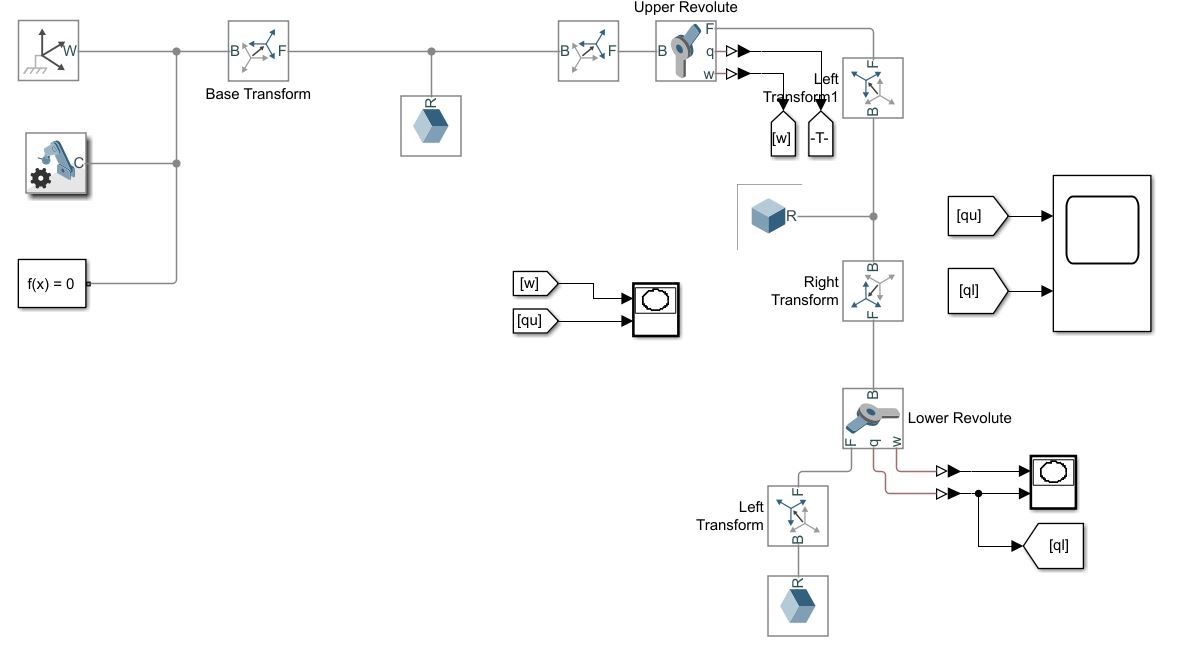
\includegraphics[width=0.7\linewidth]{model}
		\caption{Блок-схема модели}
		\label{fig:model}
	\end{figure}
	Внешний вид маятника:
	\begin{figure}[H]
		\centering
		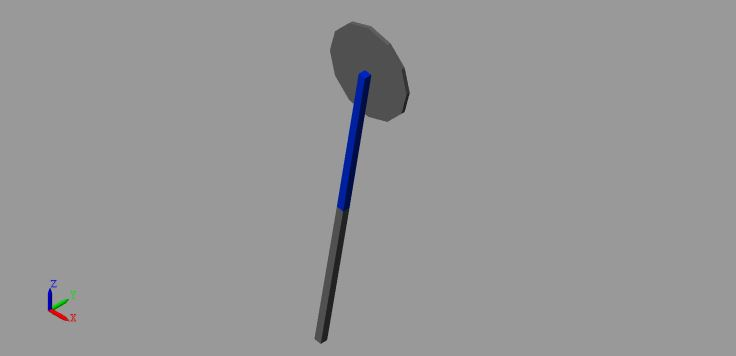
\includegraphics[width=0.7\linewidth]{3d}
		\caption{Онование -- двенадцатигранник, звенья -- параллелепипеды}
		\label{fig:3d}
	\end{figure}
	\subsection*{Моделирование свободных колебаний}
	Отклонение верхнего маятника на 10 градусов от точки равновесия, нижний маятник имеет нулевые относительные начальные условия:
	\begin{figure}[H]
		\centering
		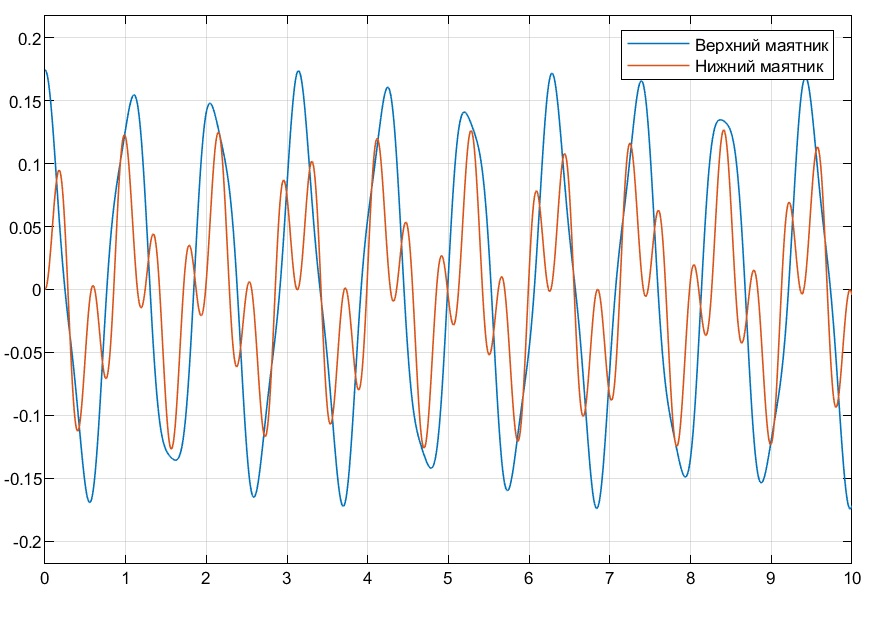
\includegraphics[width=0.7\linewidth]{up10}
		\caption{Отклонение верхнего маятника на 10 градусов от положения равновесия}
		\label{fig:up10}
	\end{figure}
	Период колебаний верхнего маятника -- 1.121 с, частота $k = 5.0$ рад/с.
	\begin{figure}[H]
		\centering
		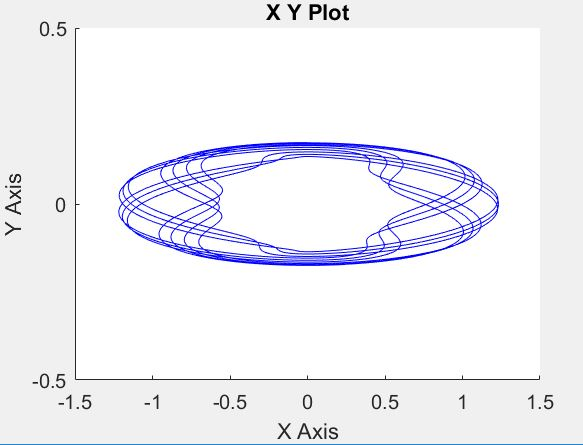
\includegraphics[width=0.7\linewidth]{upper10}
		\caption{Фазовая траектория верхнего маятника}
		\label{fig:upper10}
	\end{figure}
	\begin{figure}[H]
		\centering
		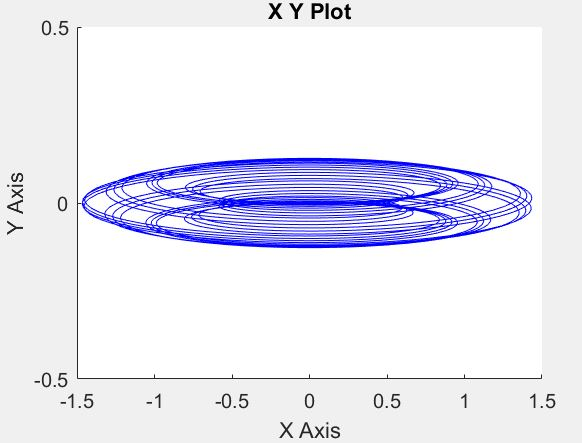
\includegraphics[width=0.7\linewidth]{lower0_10}
		\caption{Фазовая траектория нижнего маятника}
		\label{fig:lower010}
	\end{figure}
	Отклонение нижнего маятника на 10 градусов, верхний имеет нулевые начальные условия:
	\begin{figure}[H]
		\centering
		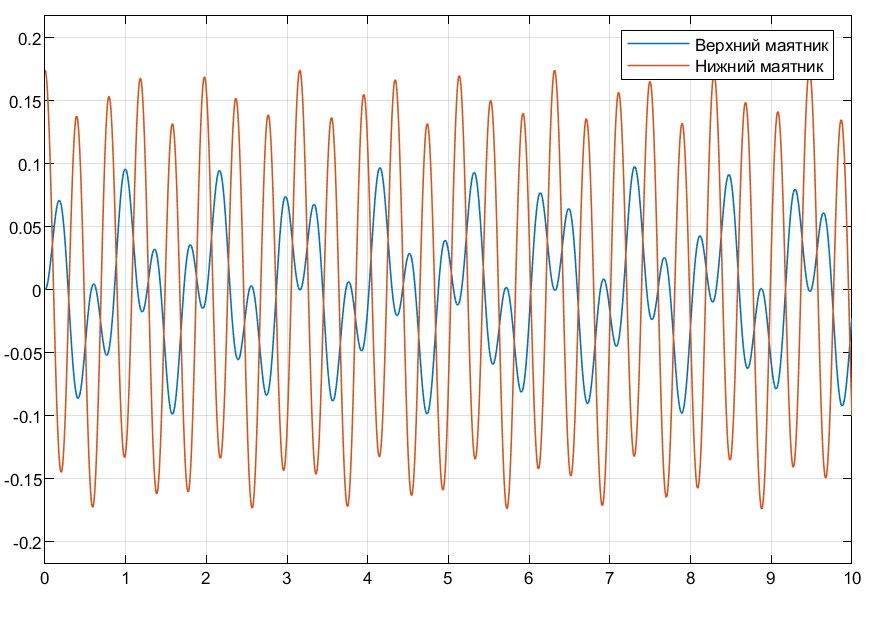
\includegraphics[width=0.7\linewidth]{down10}
		\caption{Отклонение нижнего маятника на 10 градусов}
		\label{fig:down10}
	\end{figure}
	Период колебаний -- 0.424 с, $k = 14.81$ рад/с.
	Фазовые траектории маятников:
	\begin{figure}[H]
		\centering
		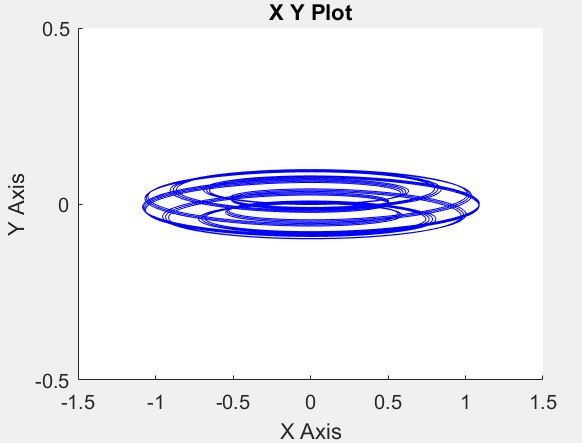
\includegraphics[width=0.7\linewidth]{upper0_10}
		\caption{Фазовая траектория верхнего маятника}
		\label{fig:upper010}
	\end{figure}
	\begin{figure}[H]
		\centering
		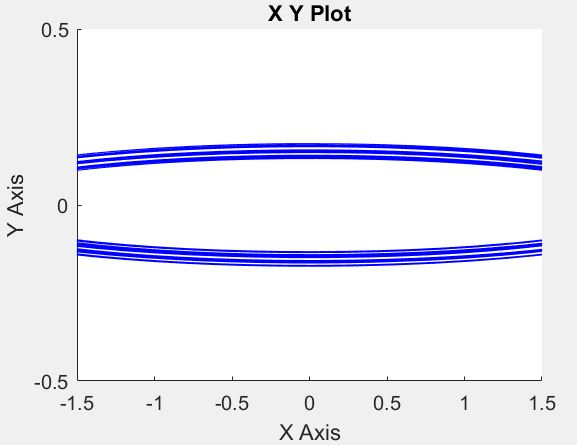
\includegraphics[width=0.7\linewidth]{lower10_0}
		\caption{Фазовая траектория нижнего маятника}
		\label{fig:lower100}
	\end{figure}
	\paragraph*{Главные колебания\\}
	Первая форма главных колебаний -- маятники качаются синхронно, колебания происходят синфазно -- оба маятника отклоняются в одну и ту же сторону:
	\begin{figure}[H]
		\centering
		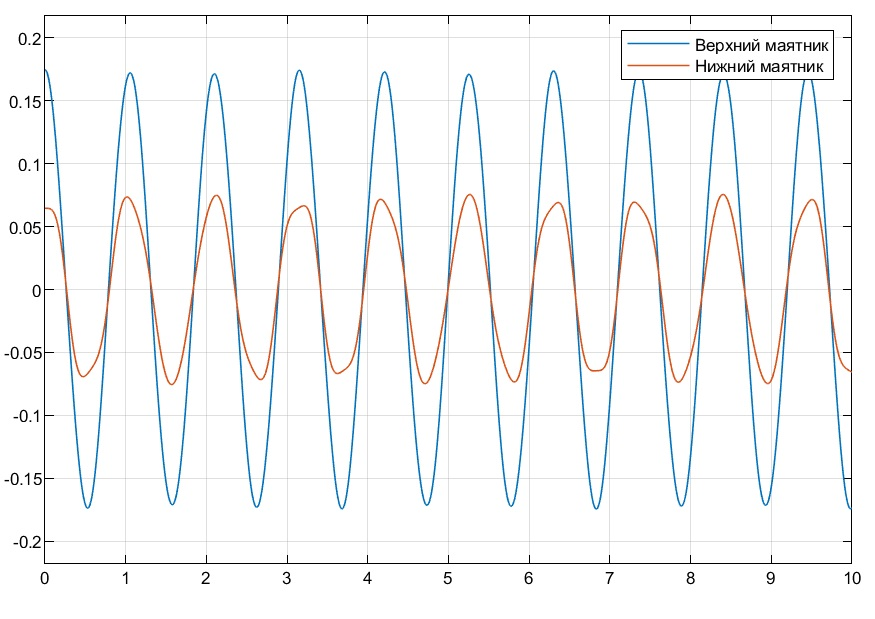
\includegraphics[width=0.7\linewidth]{sinphase10_37}
		\caption{Синфазные колебания получены при угле отклонения верхнего маятника 10 градусов, отклонение нижнего маятника -- 3.7}
		\label{fig:sinphase103}
	\end{figure}
	\begin{figure}[H]
		\centering
		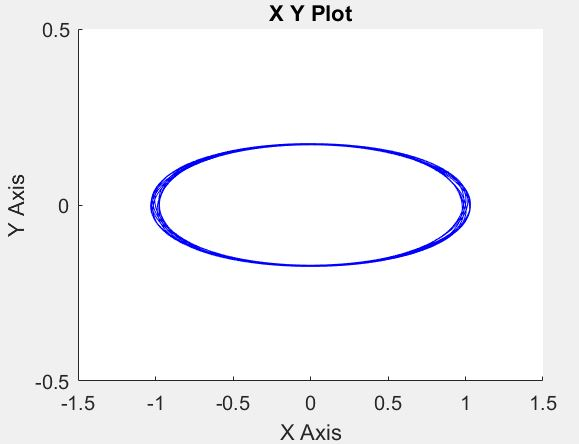
\includegraphics[width=0.7\linewidth]{sinphase_upper}
		\caption{Фазовая траектория верхнего маятника}
		\label{fig:sinphaseupper}
	\end{figure}
	\begin{figure}[H]
		\centering
		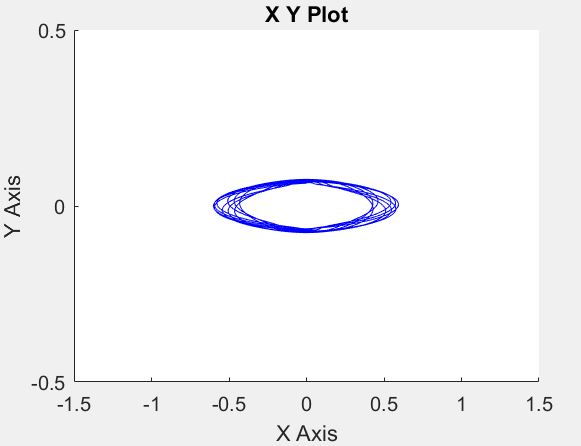
\includegraphics[width=0.7\linewidth]{sinphase_lower}
		\caption{Фазовая траектория нижнего маятника}
		\label{fig:sinphaselower}
	\end{figure}
	Период синфазных колебаний -- $\tau = 1.073$, амплитуда верхнего маятника -- 0.1745, нижнего -- 0.075. Частота $k = \frac{2\pi}{\tau} = 5.855$\\
	Вторая форма главных колебаний -- маятники отклоняются в противоположные стороны. 
	\begin{figure}[H]
		\centering
		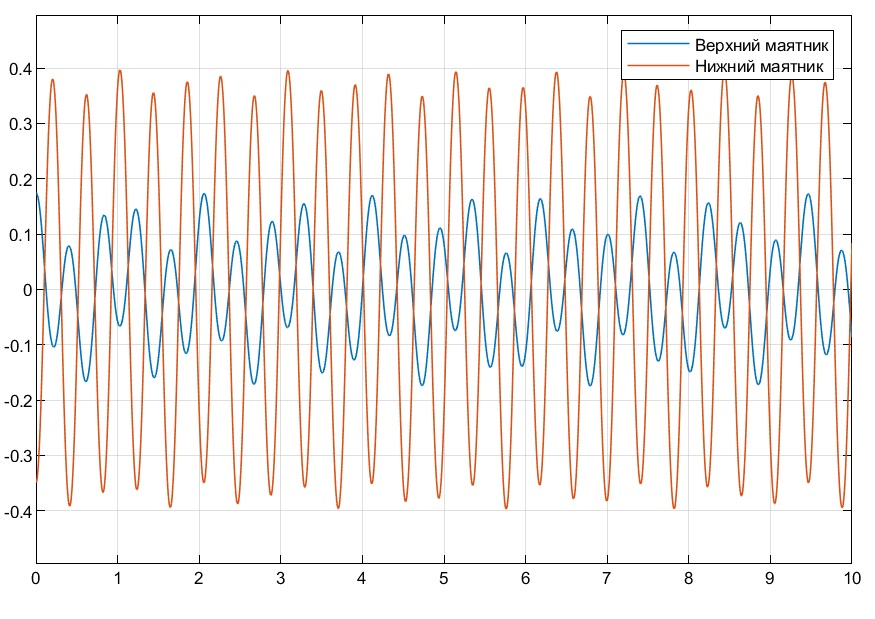
\includegraphics[width=0.7\linewidth]{gegenphase_10_-21}
		\caption{Колебания в противофазе, получены при угле отклонения верхнего маятника в 10 градусов, нижнего -- -21}
		\label{fig:gegenphase10-21}
	\end{figure}
	\begin{figure}[H]
		\centering
		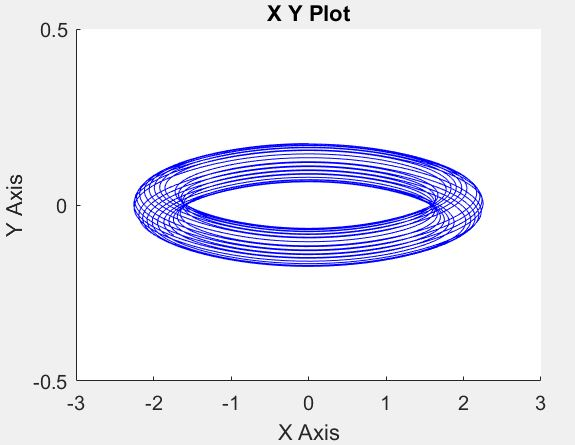
\includegraphics[width=0.7\linewidth]{gegenphase_upper}
		\caption{Фазовая траектория верхнего маятника}
		\label{fig:gegenphaseupper}
	\end{figure}
	\begin{figure}[H]
		\centering
		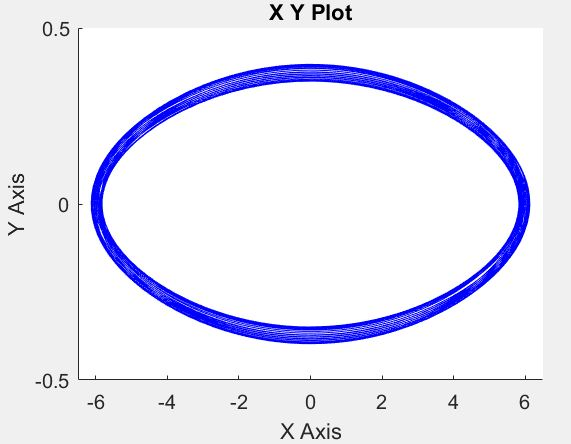
\includegraphics[width=0.7\linewidth]{gegenphase_lower}
		\caption{Фазовая траектория нижнего маятника}
		\label{fig:gegenphaselower}
	\end{figure}
	Период противофазных колебаний -- $\tau = 0.412$, амплитуда верхнего маятника -- 0.1745, нижнего -- 0.39. Частота $k = \frac{2\pi}{\tau} = 15.25$\\
	Частоты главных колебаний очень близки к парциальным частотам системы. Можно утверждать, что выполняется неравенство:
	$$k_{lower} < k_{sin} < k_{anti} < k_{upper}$$
	\subsection*{Линейный анализ и вынужденные колебания}
	\paragraph*{Линейный анализ\\}
	Для определения собственных частот системы был проведен линейный анализ системы:
	\begin{figure}[H]
		\centering
		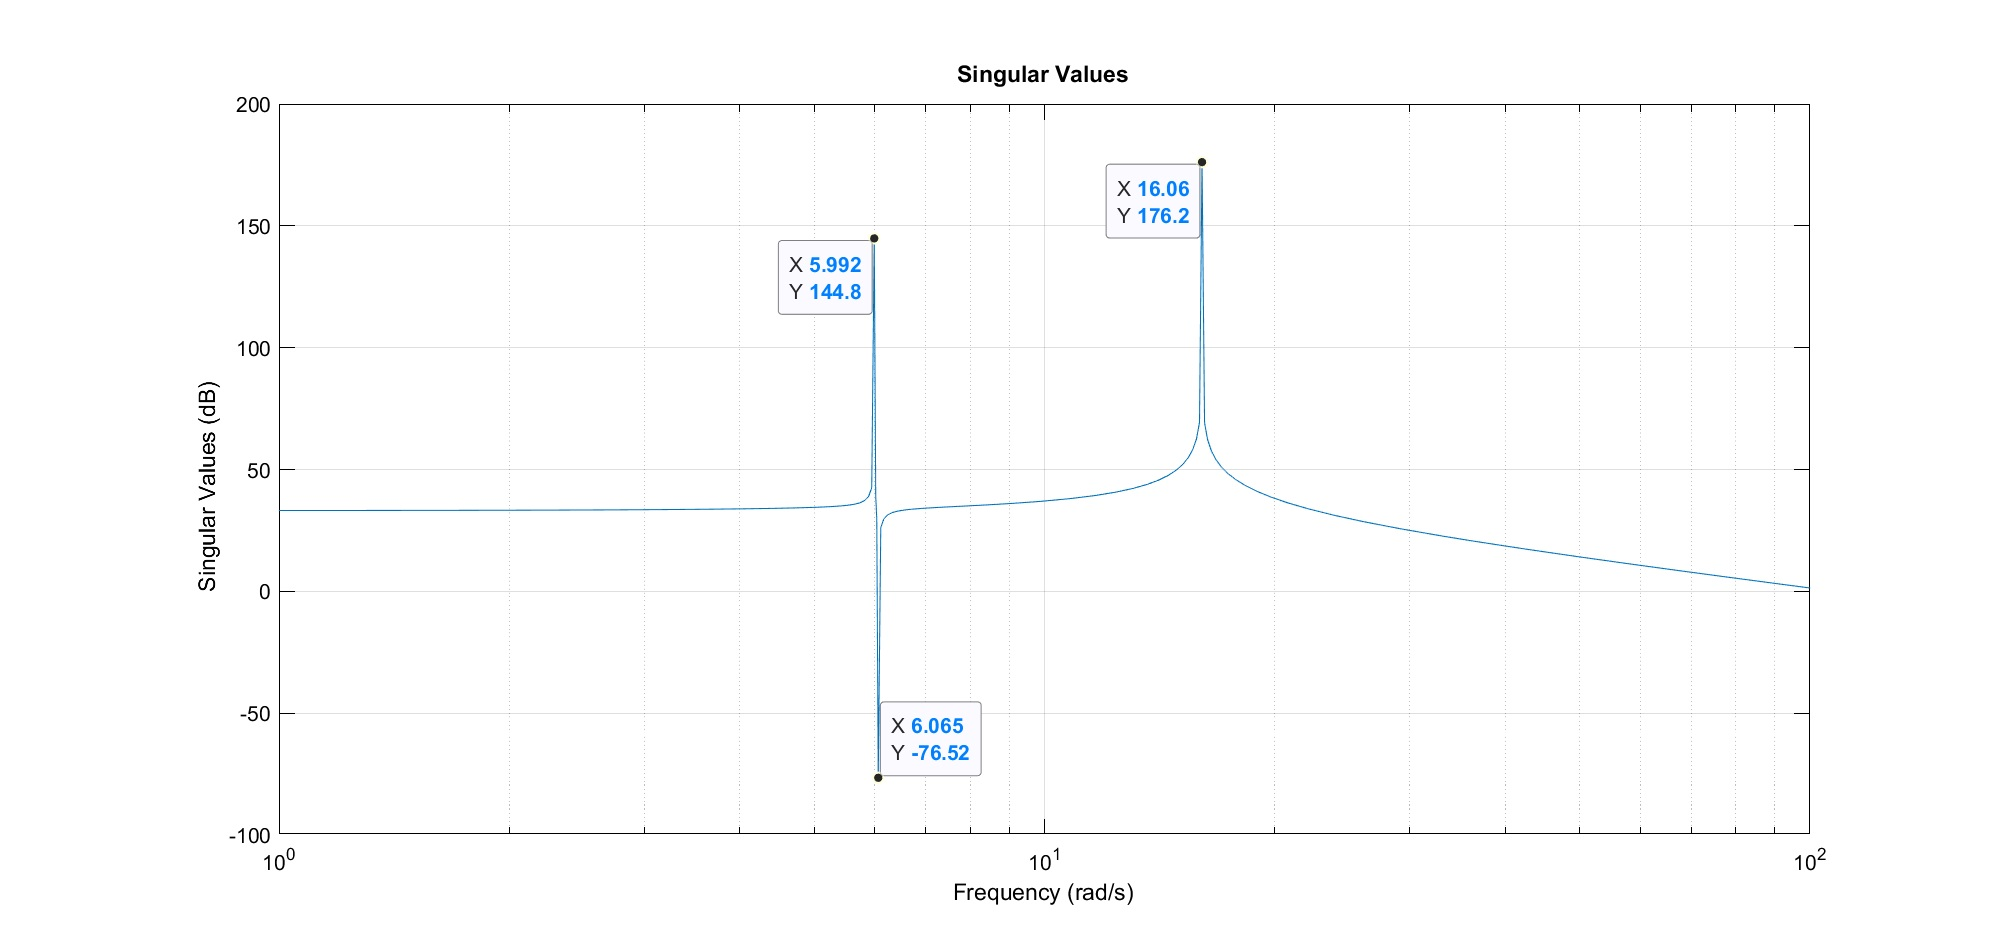
\includegraphics[width=1.2\linewidth]{SVplot}
		\caption{Singular Value Plot, $k_1 = 5.992,\ k_{gash} = 6.065,\ k_2 = 16.06$}
		\label{fig:svplot}
	\end{figure}
	После этого в схему была добавлена периодический вынуждающий момент амплитудой 0.001 Нм.
	\paragraph*{Вынужденные колебания\\}
	Колебания на первой резонансной частоте:
	\begin{figure}[H]
		\centering
		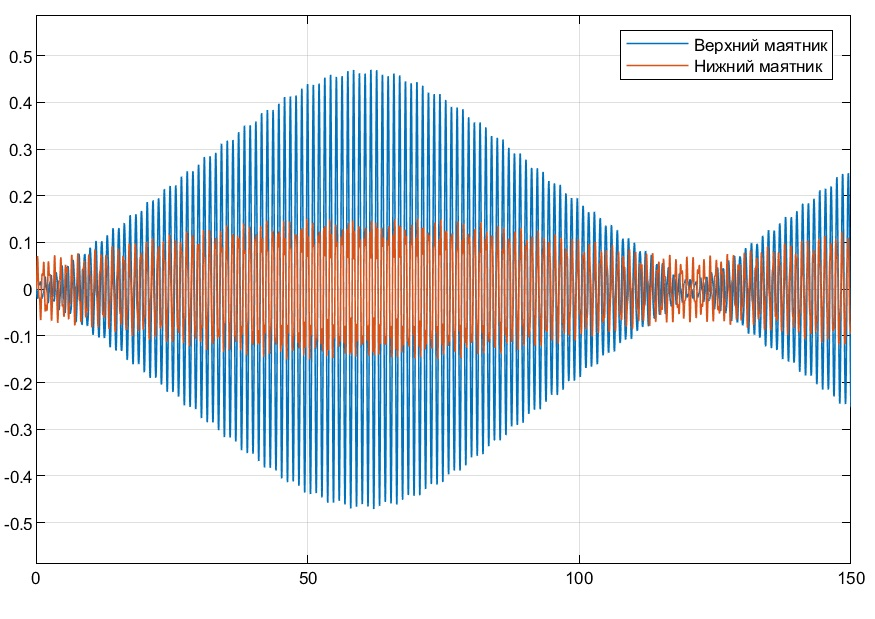
\includegraphics[width=0.7\linewidth]{k1}
		\caption{$k_1 = 5.992,\ A_{lower} = 0.1511,\ A_{upper} = 0.47$, период биений $\tau = 61.631$ с}
		\label{fig:k1}
	\end{figure}
	Колебания на частоте синфазных колебаний:
	\begin{figure}[H]
		\centering
		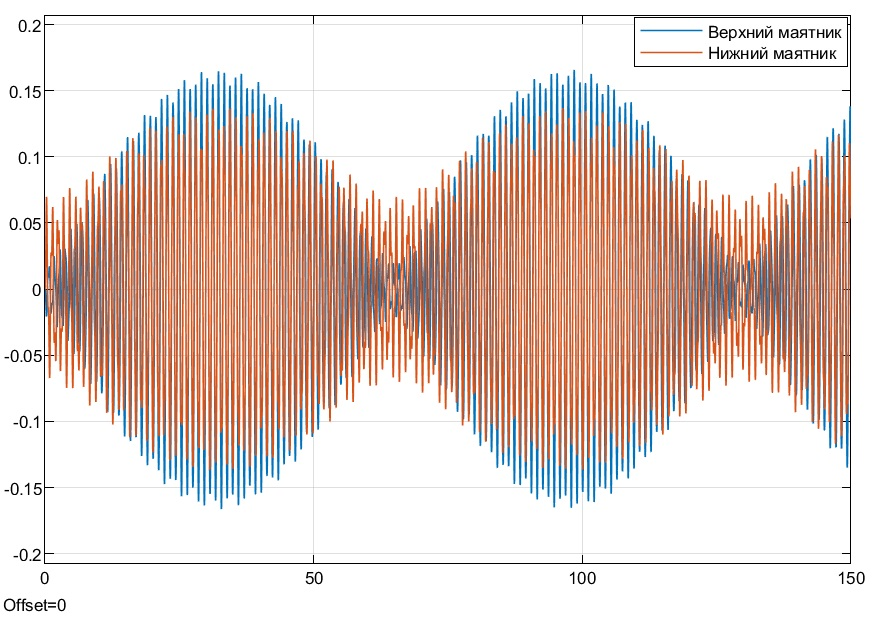
\includegraphics[width=0.7\linewidth]{ksin}
		\caption{$k_{sin} = 5.855,\ A_{lower} = 0.14,\ A_{upper} = 0.16$, период биений $\tau = 64.514$ с}
		\label{fig:ksin}
	\end{figure}
	Видно сходство колебаний на этих двух частотах, причем при колебаниях во втором случае амплитуда колебаний верхнего маятника меньше. Периоды биений примерно равны.\\
	Колебания на второй резонансной частоте:
	\begin{figure}[H]
		\centering
		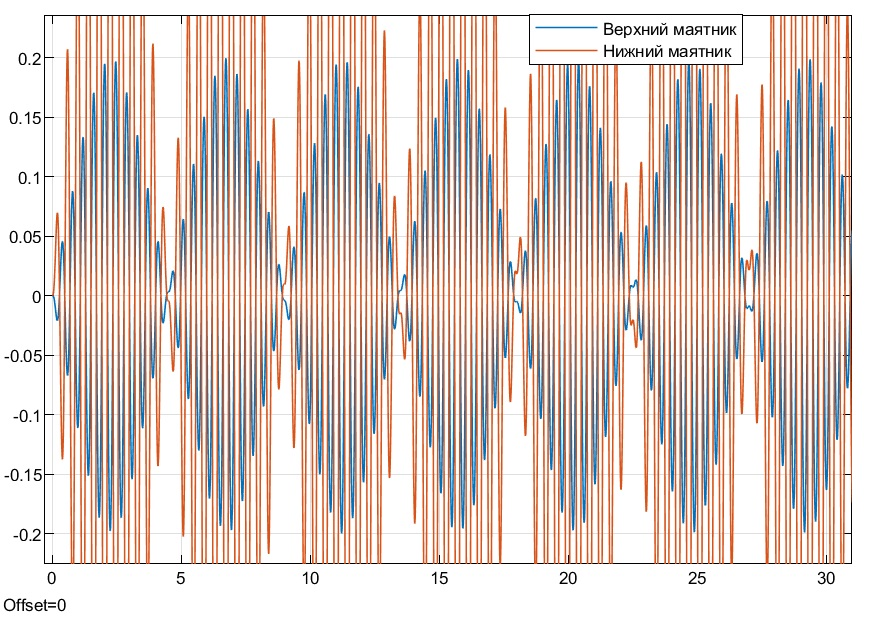
\includegraphics[width=0.7\linewidth]{k2}
		\caption{$k_2 = 16.06,\ A_{lower} = 0.62,\ A_{upper} = 0.1993$, период биений $\tau = 4.503$ с}
		\label{fig:k2}
	\end{figure}
	Если на первой резонансной частоте резко возрастает амплитуда колебаний верхнего маятника, то на второй резонансной частоте резко возрастает амплитуда колебаний нижнего маятника, уменьшается период биений.\\
	Колебания на частоте противофазных колебаний:
	\begin{figure}[H]
		\centering
		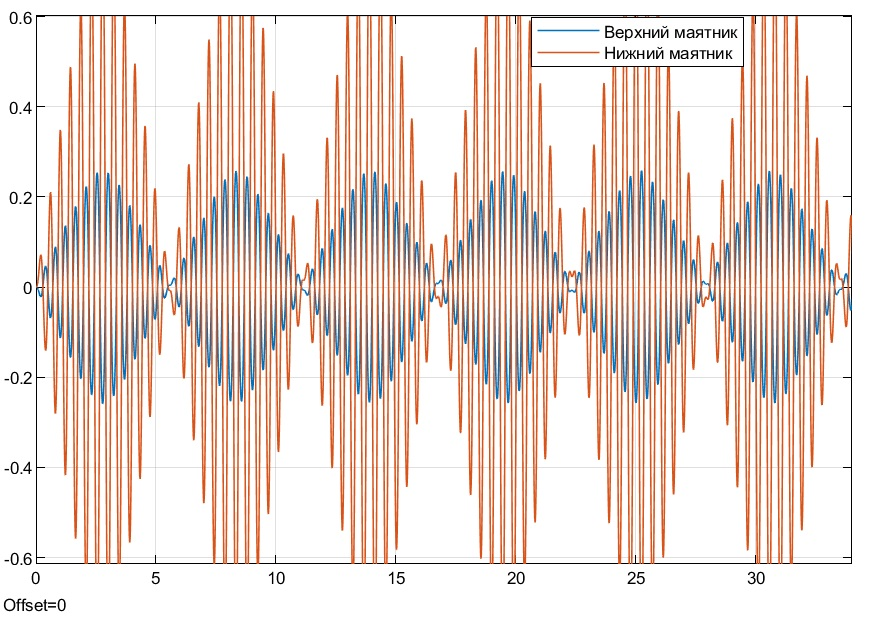
\includegraphics[width=0.7\linewidth]{kgegen}
		\caption{$k_{gegen} = 15.25,\ A_{lower} = 0.8,\ A_{upper} = 0.2582$, период биений $\tau = 5.771$ с}
		\label{fig:kgegen}
	\end{figure}
	Видно сходство с колебаниями на второй резонансной частоте, но период биений и амплитуда колебаний обоих маятников больше, чем в предыдущем случае.\\
	Колебания на частоте гашения:
	\begin{figure}[H]
		\centering
		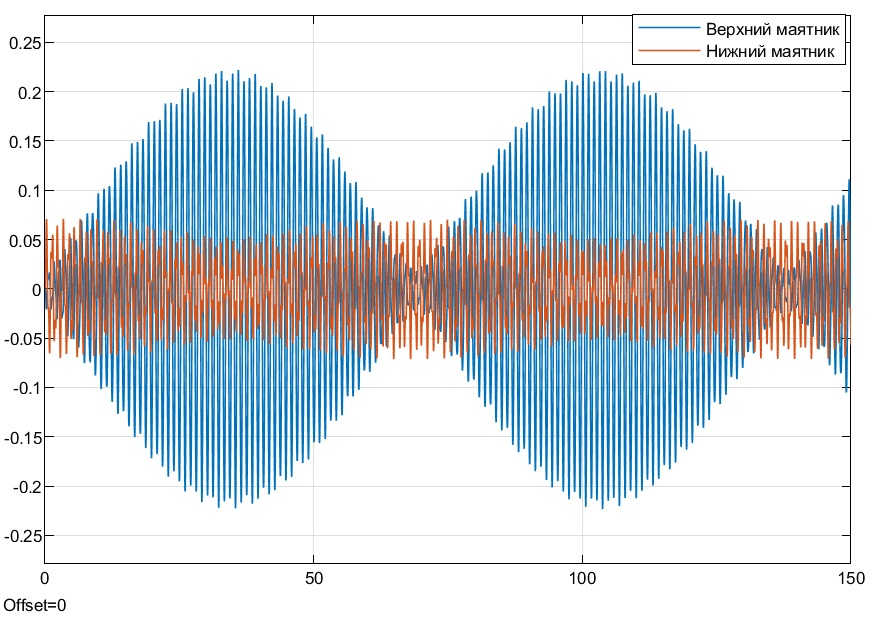
\includegraphics[width=0.7\linewidth]{kgash}
		\caption{$k_{gash} = 6.065,\ A_{lower} = 0.071,\ A_{upper} = 0.22$, период биений $\tau = 69.476$ с}
		\label{fig:kgash}
	\end{figure}
	Как видно из графика, происходит периодическое уменьшение амплитуды колебаний нижнего маятника до 0.05, но полного гашения не происзодит. Вместе с уменьшением амплитуды нижнего маятника происходит возрастание амплитуды верхнего.	
\end{document}